\documentclass[12pt,a4paper]{article}
\usepackage[utf8]{inputenc}
\usepackage[spanish]{babel}
\usepackage{amsmath}
\usepackage{amsfonts}
\usepackage{amssymb}
\usepackage{graphicx}
\usepackage[left=2cm,right=2cm,top=2cm,bottom=2cm]{geometry}
\author{CINEMATICA DIRECTE E INVERSA EN MANIPULADORES.\\Enciso Guerrero Benjamin Salvador\\
Carlos Enrrique Moran Garabito\\
Cinematica De Robots }
\title{UNIVERSIDAD POLITECNICA DE LA ZONA METROPOLITANA DE GUADALAJARA.}
\begin{document}
\maketitle

\includegraphics[scale=1.8]{upzmgg.jpg} 
\newpage
CINEMATICA DIRECTE E INVERSA EN MANIPULADORES.
\\\\
En robots paralelos, la cinemática inversa consiste en encontrarlas variables de las juntas activas y pasivas en función de las coordenadas del efector final del robot y puede ser utilizada para controlarla posición del efector final. El modelo cinemático de este tipo de robots tiene ecuaciones algebraicas con múltiples soluciones.
\\\\
En la cinemática directa de robots paralelos el problema es determinar la posición del efector final en función de las juntas activas. En general, la solución a este problema no es única, de ahí que la cinemática ha sido objeto de una intensa investigación. Sin embargo, la solución del polinomio no asegura la correcta evolución de las variables de las juntas activas y no considera a las juntas pasivas, al ejecutar una tarea dada. Por otro lado, no hay algoritmo conocido que permita la fácil determinación de una postura única para la plataforma móvil.
\\\\
 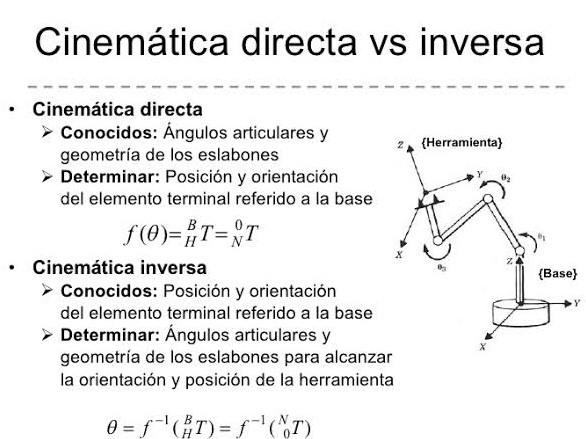
\includegraphics[scale=1]{CINE.jpg} 
\\Figura 1.1 Diferencia entre directa e inverza
\\\\
Es importante hacer hincapié en el problema del resultado de la cinemática directa por polinomio. El cálculo puede implicar un gran número de operaciones y por lo tanto puede ser muy sensible a errores numéricos de redondeo; por esta razón la comprobación de la validez de las soluciones con la cinemática inversa es normalmente necesaria.
\\\\
La solución de la cinemática directa e inversa, utilizando la integración de la cinemática diferencial, es particularmente importante para los manipuladores de cadenas cinemáticas cerradas cuyas soluciones no existen, son difíciles de obtener, o son demasiado complejas para ser tratadas; el trabajo de Campos, A., R. Guenther, y D. Martins, sobre robots redundantes o paralelos, constituye un buen ejemplo de esto.
\\\\
Chung aborda la cinemática de robots manipuladores seriales redundantes planos, utilizando cadenas virtuales y subcadenas virtuales, para resolver el problema de la cinemática inversa. Chung define a un eslabón virtual como un enlace ficticio que conecta a dos articulaciones. 
\\\\
Las ventajas son que reduce la carga de cómputo y logra la manipulación a nivel general mediante la obtención óptima de los ángulos. Entre las desventajas que presenta esta estrategia de análisis se puede mencionar que sólo se aplican a robots seriales planos, es complicado utilizar el método en manipuladores paralelos y tampoco se consideran las velocidades lineales y angulares del robot.
\\\\
angulares del robot.
Toshio describe al brazo virtual como un manipulador que tiene la misma estructura cinemática de un manipulador real. Su teoría se basa en un sistema que denomina distribuido y que es la representación de la cinemática del manipulador. Así mismo, utiliza la propagación hacia atrás de redes neuronales. 
\\\\
Entre las ventajas del método se pueden mencionar varias; cada subsistema puede trabajar totalmente autónomo, el movimiento de la articulación del manipulador redundante se puede calcular de una manera paralela y distribuida y la redundancia cinemática del manipulador puede ser utilizada positivamente usando sub-brazos virtuales. 
\\\\
Algunas desventajas del modelo propuesto por Toshio son que sólo se puede utilizar en robots seriales redundantes planos, asimismo, no toma en cuenta las velocidades lineales y angulares del robot.
\\\\
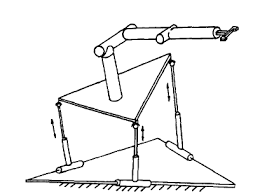
\includegraphics[scale=1]{POSTURA DEL ROBOT 3RRR.png} 
FIGURA 1.1
\\\\
El modelo de un manipulador paralelo delta plano de configuración 3RRR-(RRR)v y por el otro, el modelo de su cadena virtual serial (RRR)v. 
\\\\
Esta retroalimentación es llamada "actuación virtual indirecta". El enfoque propuesto garantiza que cuando el efector final de la cadena virtual serial (RRR)v es controlado alrededor de una trayectoria, el efector final del robot paralelo plano 3RRR también sigue dicha trayectoria; esto se debe a que comparten el mismo punto de análisis. Los resultados muestran que es posible controlar un robot paralelo delta plano 3RRR-(RRR)v a partir de controlar la cadena virtual (RRR)v.



\end{document}